\documentclass[conference]{IEEEtran}
\IEEEoverridecommandlockouts
% The preceding line is only needed to identify funding in the first footnote. If that is unneeded, please comment it out.
\usepackage{cite}
\usepackage{amsmath,amssymb,amsfonts}
% \usepackage{algorithmic}
\usepackage[ruled, vlined, linesnumbered]{algorithm2e}
\usepackage{mhchem}
\usepackage{graphicx}
\usepackage{textcomp}
\usepackage{xcolor}
\usepackage{booktabs}

\usepackage{subfigure}
\usepackage{hyperref}
\usepackage{makecell}
\usepackage{adjustbox}

\newcommand{\note}[1]{{\color{blue} #1}}
\newcommand{\ZY}[1]{{\color{purple}[ZY: #1]}}

\newcommand{\phoenix}{\textsc{Phoenix}}
\newcommand{\qiskit}{\textsc{Qiskit}}
\newcommand{\tket}{\textsc{TKet}}
\newcommand{\tetris}{\textsc{Tetris}}
\newcommand{\paulihedral}{\textsc{Paulihedral}}
\newcommand{\pcaost}{\textsc{PCOAST}}
\newcommand{\twoqan}{\textsc{2QAN}}


\SetAlFnt{\small}
% \SetAlCapFnt{\small}



% \newcommand{\note}{\underline}

\hypersetup{hidelinks}
% \hypersetup{draft}

\def\BibTeX{{\rm B\kern-.05em{\sc i\kern-.025em b}\kern-.08em
    T\kern-.1667em\lower.7ex\hbox{E}\kern-.125emX}}
\begin{document}

% \title{Conference Paper Title*\\
% {\footnotesize \textsuperscript{*}Note: Sub-titles are not captured in Xplore and
% should not be used}
% \thanks{Identify applicable funding agency here. If none, delete this.}
% }

\title{\phoenix: Pauli-based High-level Optimization Engine for Instruction Execution on NISQ Devices}

% VQA Programs Synthesis by Clifford Formalism



% \author{
%     \IEEEauthorblockN{Zhaohui Yang}
%     \IEEEauthorblockA{\textit{Department of Electrical \& Computer Engineering} \\
%     \textit{University of Arizona}\\
%     Tucson, AZ, USA\\
%     zhy@arizona.edu}
% }


% \author{
%     \IEEEauthorblockN{Zhaohui Yang\IEEEauthorrefmark{1}, David Ding\IEEEauthorrefmark{2}, Jianxin Chen\IEEEauthorrefmark{3}, Yuan Xie\IEEEauthorrefmark{1}}
    
%     \IEEEauthorblockA{\textit{\IEEEauthorrefmark{1}Department of Electronic and Computer Engineering, The Hong Kong University of Science and Technology, Hong Kong}}

%     \IEEEauthorblockA{\textit{\IEEEauthorrefmark{2} Yau Mathematical Sciences Center, Tsinghua University, Beijing, China}}

%     \IEEEauthorblockA{\textit{\IEEEauthorrefmark{3}Department of Computer Science and Technology, Tsinghua University, Beijing, China}}


%     % \IEEEauthorblockA{\{zhaohui\}@ucsb.edu, }
% }


\maketitle


\begin{abstract}
    Quantum computing ...

    We propose a Pauli-based High-level Optimization ENgine for Instruction eXecution (\phoenix) of Hamiltonian simulation programs on NISQ devices

    
    
\end{abstract}

% \begin{IEEEkeywords}
% Entanglement distribution, network protocol design, platform-as-a-service, quantum communication, quantum internet service provider, quantum network, reconfigurable network architecture, routing, software-defined network.
% \end{IEEEkeywords}



%%%%%%%%%%%%%%%%%%%%%%%%%%%%%%%%%%%%%%%%%%%%%%%%
% Introduction
%%%%%%%%%%%%%%%%%%%%%%%%%%%%%%%%%%%%%%%%%%%%%%%%

\section{Introduction}

    Quantum computing ...
    

    % Some recent demonstrative experiments of entanglement distribution have begun to use CV entangled photons \cite{zhang2008distribution}, especially for long-distance scenarios.


    % The rest of this paper is structured as follows. In Sec. \ref{sec:2:resutls}, we firstly describe the hardware infrastructures and their re-constructing approaches on basis of the existing fiber-based network at the University of Arizona (UA), and then explain how the QISP is implemented under a reconfigurable framework. Field-test evaluation results are also included in this section. We summarize our work in Sec. \ref{sec:3:discussion} with analyses of current limitations and future work directions. In Sec. \ref{sec:4:methods}, we will see in more detail the Quagent's architecture and the entanglement source characterization methods.



%%%%%%%%%%%%%%%%%%%%%%%%%%%%%%%%%%%%%%%%%%%%%%%%
% Motivation
%%%%%%%%%%%%%%%%%%%%%%%%%%%%%%%%%%%%%%%%%%%%%%%%

\section{Motivation}

\ZY{Motivation and preliminary knowledge}


\section{Our Propsal: \phoenix}

\subsection{Overall framework}

\subsection{BSF simplification for each IR group}


    \begin{algorithm}[tbp]
        \SetAlgoLined
        \caption{Pauli Strings Simplification in BSF}
        \label{algo:simplification}
        \SetKwInOut{Input}{Input}
        \SetKwInOut{Output}{Output}
        \SetKwBlock{Assumption}{Assumption}{}
    
        % \Input{Pauli strings with corresponding coefficients (\textit{pls}, \textit{coes})}
        \Input{Pauli strings list \textit{pls}}
        \Output{Reconfigured circuit components list \textit{cfg}}
    
        % \tcp{Following pseudocode only involves transformation on pls while omitting coes WLOG}
        \BlankLine
        \textit{cfg} $ \gets \emptyset $;\quad
        \textit{bsf} $ \gets \textsc{BSF}$(\textit{pls});\quad
        \textit{cliffs\_with\_locals} $\gets \emptyset$\; %\tcp*{Cliffords with local Paulis}
        % $ n \gets $ \textit{bsf}.\textsc{numQubits}()\;
        \While{bsf.\textsc{totalWeight()} $>$ 2}{
            \textit{local\_bsf} $\gets$ \textit{bsf}.\textsc{popLocalPaulis}()\; 
            % $ C \gets \emptyset$;\quad
            % $ B \gets \emptyset$;\quad
    
            $ C \gets \emptyset$ \tcp*{Clifford2Q candidates}
            $ B \gets \emptyset$ \tcp*{Each element of $B$ results from applying each Clifford2Q candidate on \textit{bsf}}
            \textit{costs} $\gets \emptyset$ \tcp*{Cost functions calculated on each element of $B$}
            \For{cg \textbf{in} \textsc{CLIFFORD\_2Q\_SET}}{
                \For{i, j \textbf{in} $ \textsc{combinations}(\textsc{range}(n), 2) $}{
                    \textit{cliff} $\gets$ \textit{cg}.\textsc{on}$ (i, j) $ \tcp*{qubits acted on}
                    \textit{bsf}$'$ $\gets$ \textit{bsf}.\textsc{applyClifford2Q}(\textit{cliff})\;
                    \textit{cost} $\gets$ \textsc{calculateBSFCost}(\textit{bsf}$'$)\;
                    $ C.\textsc{append}$(\textit{cliff})\;
                    $ B.\textsc{append}$(\textit{bsf}$'$)\;
                    \textit{costs}.\textsc{append}(\textit{cost})\;
                }
            }
            % \textit{bsf} $\gets$ \textit{B}[\textit{costs}.\textsc{index}(\textit{min}(\textit{costs}))]\;
            % \textit{cliff} $\gets$ \textit{C}[\textit{costs}.\textsc{index}(\textit{min}(\textit{costs}))]\;
            \textit{bsf} $ \gets \textsc{BSFWithMinCost} (B, \textit{costs}) $\;
            \textit{cliff} $ \gets \textsc{CliffordWithMinCost} (C, \textit{costs}) $\;
            \textit{cliffs\_with\_locals}.\textsc{append}((\textit{cliff}, \textit{local\_bsf}))\;
        }
        \BlankLine
        \textit{cfg}.\textsc{append}(\textit{bsf})\;
        \For{cliff, local\_bsf \textbf{in} cliffs\_with\_locals}{
            \tcp{Clifford2Q operators are added as conjugations, with local Pauli strings peeled before each epoch}
            \textit{cfg}.\textsc{prepend}(\textit{cliff})\;
            \textit{cfg}.\textsc{append}(\textit{local\_bsf})\;
            \textit{cfg}.\textsc{append}(\textit{cliff})\;
        }
    
    \end{algorithm}


\subsection{Ordering of IR groups}


%%%%%%%%%%%%%%%%%%%%%%%%%%%%%%%%%%%%%%%%%%%%%%%%%%%%%%%%%
% Evaluation
%%%%%%%%%%%%%%%%%%%%%%%%%%%%%%%%%%%%%%%%%%%%%%%%%%%%%%%%%

\section{Evaluation}


\subsection{Experimental settings}


\begin{table}[tbp]
    \centering
    \caption{UCCSD benchmark suite.}
    \setlength{\tabcolsep}{4.2pt}
    % \fontsize{5}{5}\selectfont
    \scalebox{0.876}{
        \begin{tabular}{|l|r|r|r|r|r|r|r|}
    % \toprule
    \hline
    \textbf{Benchmark} & \textbf{\#Qubit} & \textbf{\#Pauli} & $\mathbf{w_{\max}}$ & \textbf{\#Gate} & \textbf{\#CNOT}  & \textbf{Depth} & \textbf{Depth-2Q} \\
    % \midrule
    \hline
    CH2\_cmplt\_BK & 14 & 1488 & 10 & 37780 & 19574 & 23568 & 19399 \\
    \hline
    CH2\_cmplt\_JW & 14 & 1488 & 14 & 34280 & 21072 & 23700 & 19749 \\
    \hline
    CH2\_frz\_BK & 12 & 828 & 10 & 19880 & 10228 & 12559 & 10174 \\
    \hline
    CH2\_frz\_JW & 12 & 828 & 12 & 17658 & 10344 & 11914 & 9706 \\
    \hline
    H2O\_cmplt\_BK & 14 & 1000 & 10 & 25238 & 13108 & 15797 & 12976 \\
    \hline
    H2O\_cmplt\_JW & 14 & 1000 & 14 & 23210 & 14360 & 16264 & 13576 \\
    \hline
    H2O\_frz\_BK & 12 & 640 & 10 & 15624 & 8004 & 9691 & 7934 \\
    \hline
    H2O\_frz\_JW & 12 & 640 & 12 & 13704 & 8064 & 9332 & 7613 \\
    \hline
    LiH\_cmplt\_BK & 12 & 640 & 10 & 16762 & 8680 & 10509 & 8637 \\
    \hline
    LiH\_cmplt\_JW & 12 & 640 & 12 & 13700 & 8064 & 9342 & 7616 \\
    \hline
    LiH\_frz\_BK & 10 & 144 & 9 & 2890 & 1442 & 1868 & 1438 \\
    \hline
    LiH\_frz\_JW & 10 & 144 & 10 & 2850 & 1616 & 1985 & 1576 \\
    \hline
    NH\_cmplt\_BK & 12 & 640 & 10 & 15624 & 8004 & 9691 & 7934 \\
    \hline
    NH\_cmplt\_JW & 12 & 640 & 12 & 13704 & 8064 & 9332 & 7613 \\
    \hline
    NH\_frz\_BK & 10 & 360 & 9 & 8303 & 4178 & 5214 & 4160 \\
    \hline
    NH\_frz\_JW & 10 & 360 & 10 & 7046 & 3896 & 4640 & 3674 \\
    % \bottomrule
    \hline
\end{tabular}    

    }
    \label{tab:uccsd}
    
\end{table}

\subsection{Benchmarks}


\subsubsection{Metrics}

\subsubsection{Baselines}

\begin{itemize}
    \item \tket
    \item \paulihedral
    \item \tetris
\end{itemize}



\subsection{Logical-level compilation}


\begin{figure}[tbp]
    \centering
    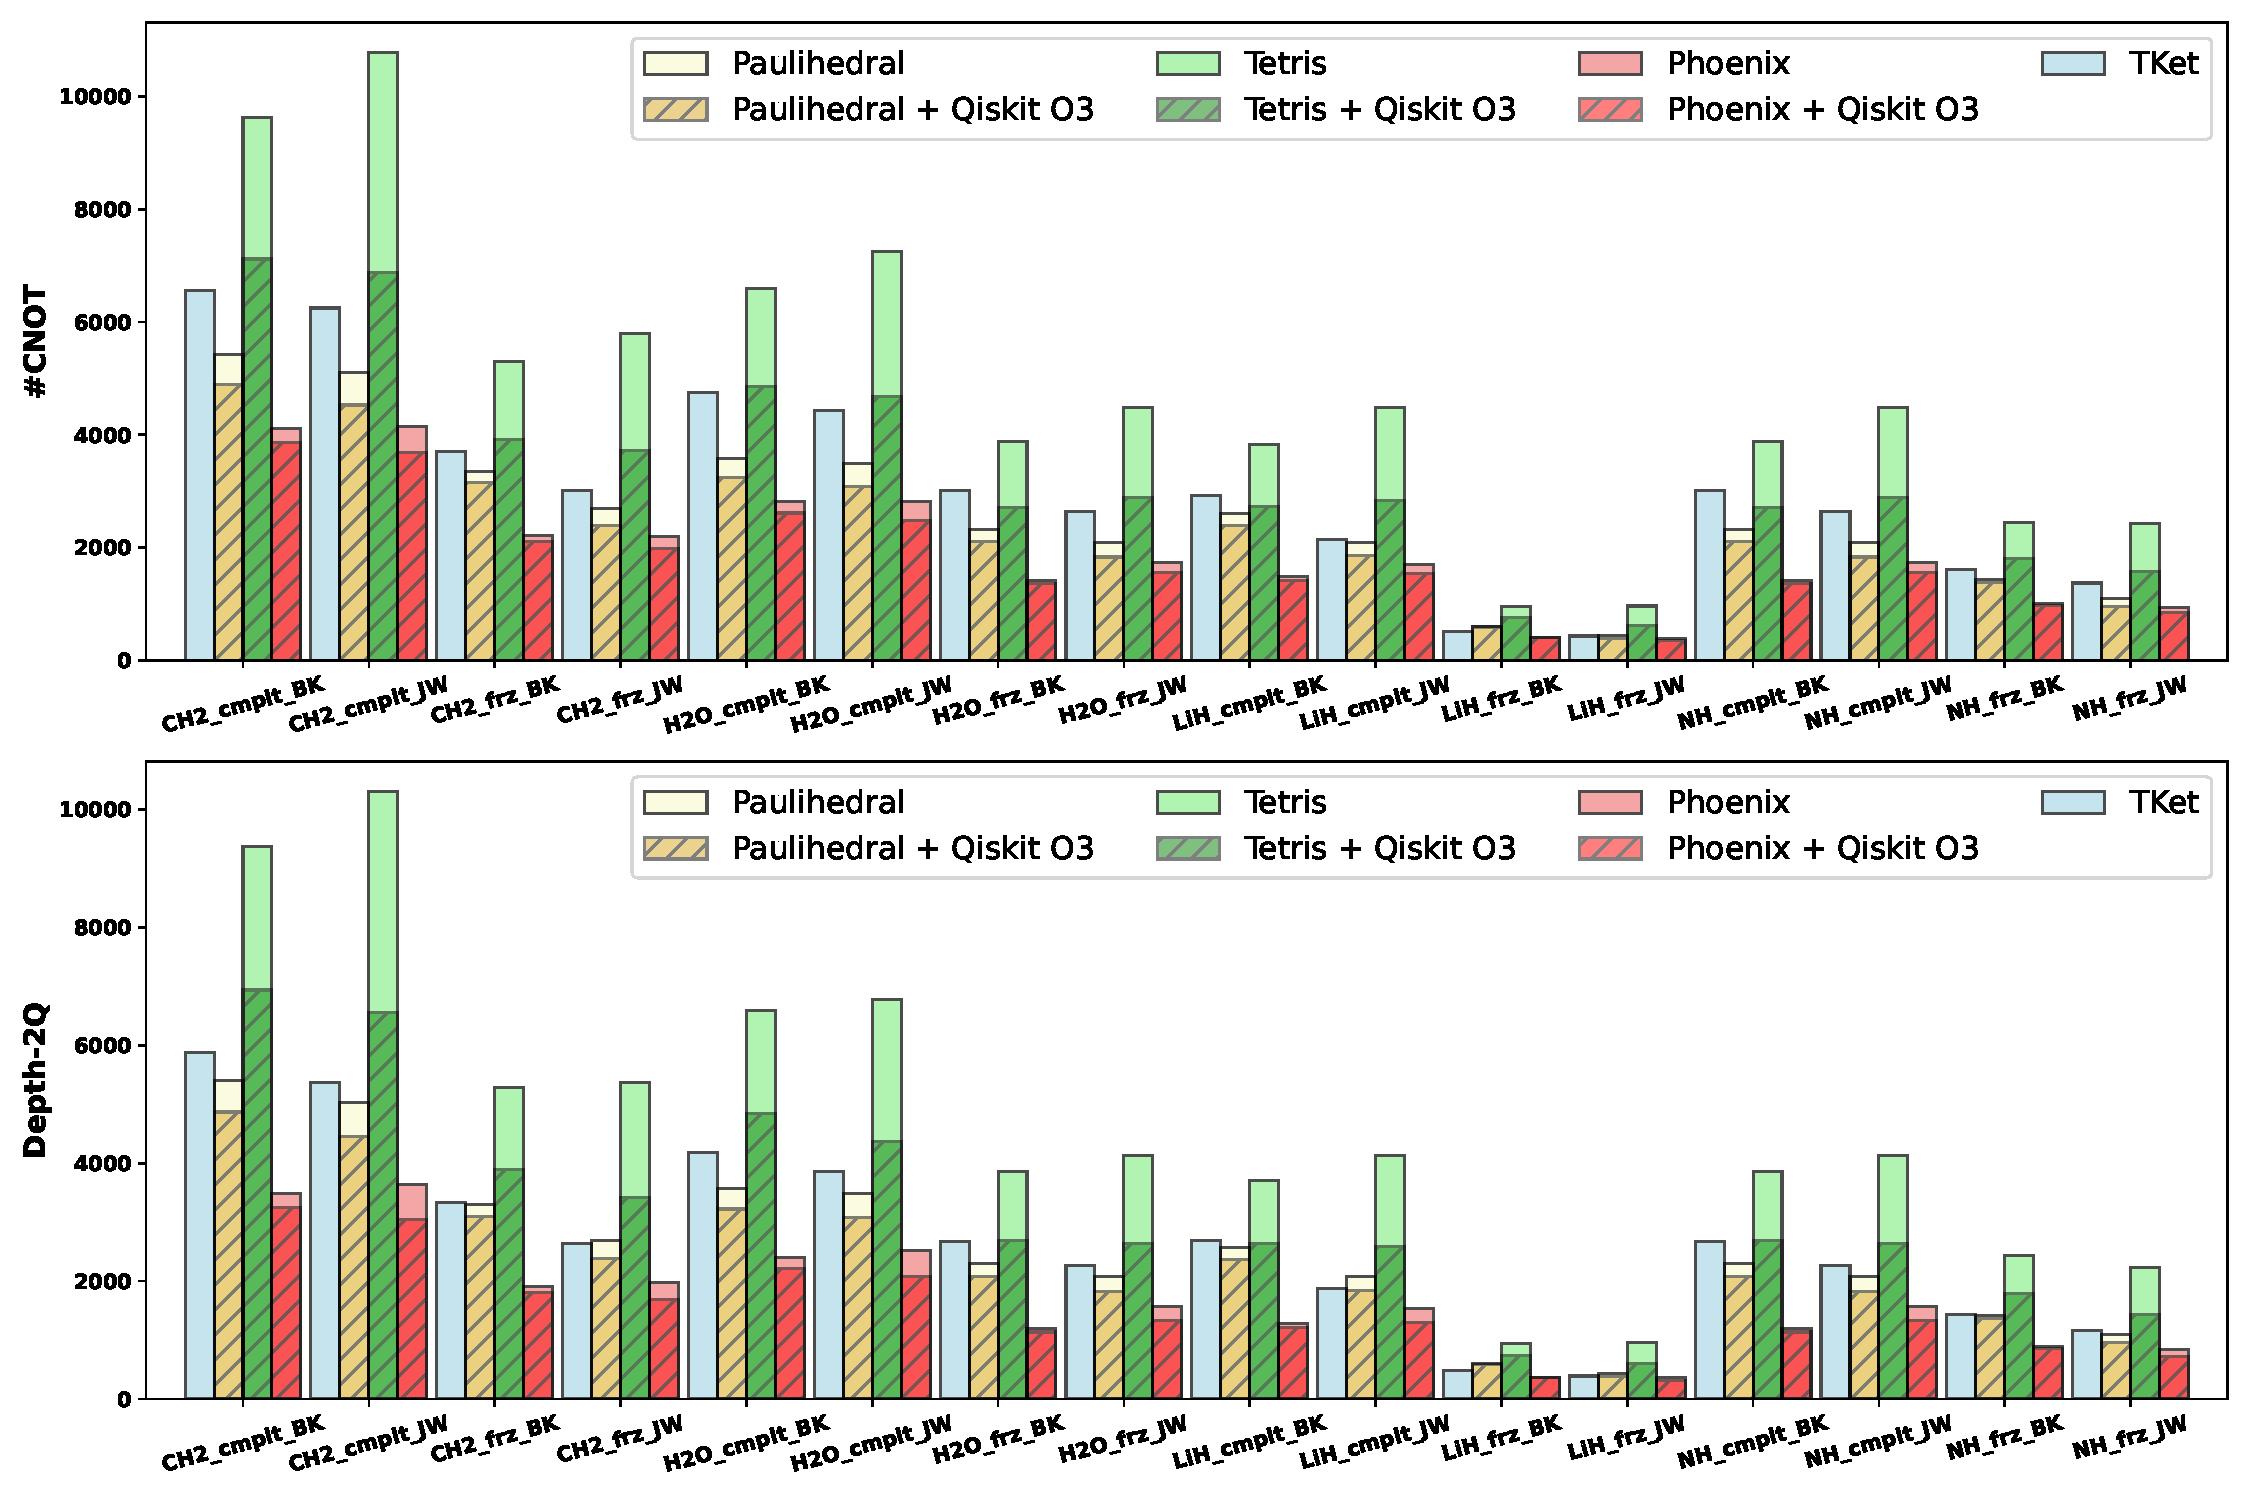
\includegraphics[width=\columnwidth]{figures/all2all.pdf}
    \caption{Bechmarking on logical-level synthesis (all2all topology)}
    \label{fig:all2all}
\end{figure}


\subsection{Breakdown analysis}


\subsection{QAOA benchmarking}



\begin{figure}[tbp]
    \centering
    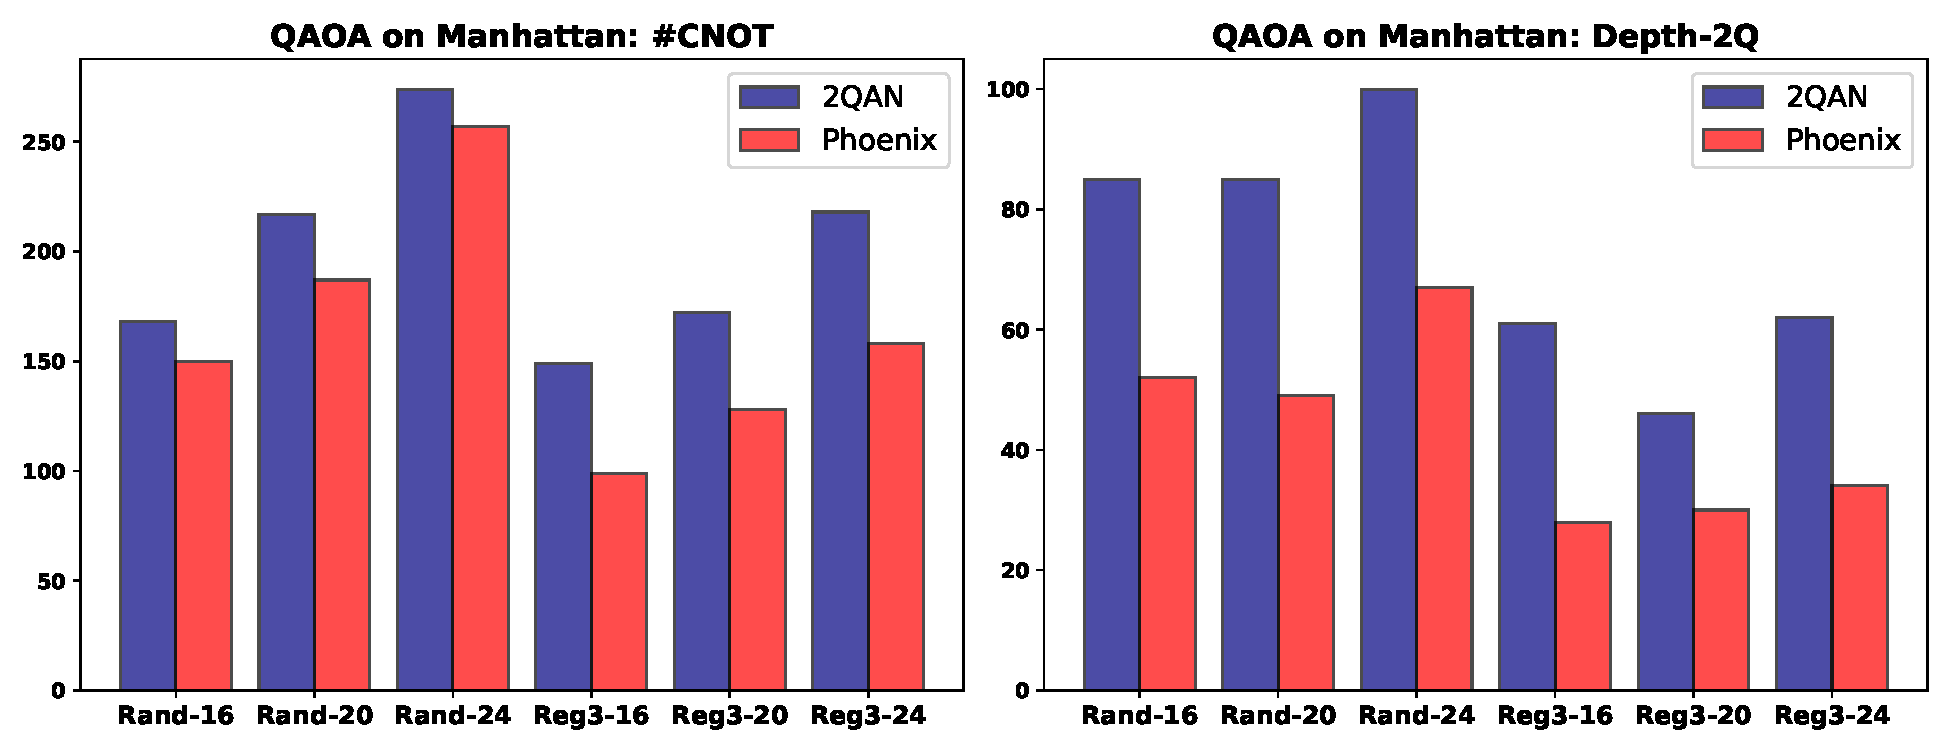
\includegraphics[width=\columnwidth]{figures/qaoa.pdf}
    \caption{QAOA benchmarking}
    \label{fig:qaoa}
\end{figure}



\begin{table*}[btp]
    \centering
    \caption{QAOA benchmarking versus 2QAN.}
    \scalebox{1}{
        \inpute{tables/qaoa.tex}
    }
    \lable{tab:qaoa}
\end{table*}


\subsection{Hardware-aware compilation}


\begin{figure}[tbp]
    \centering
    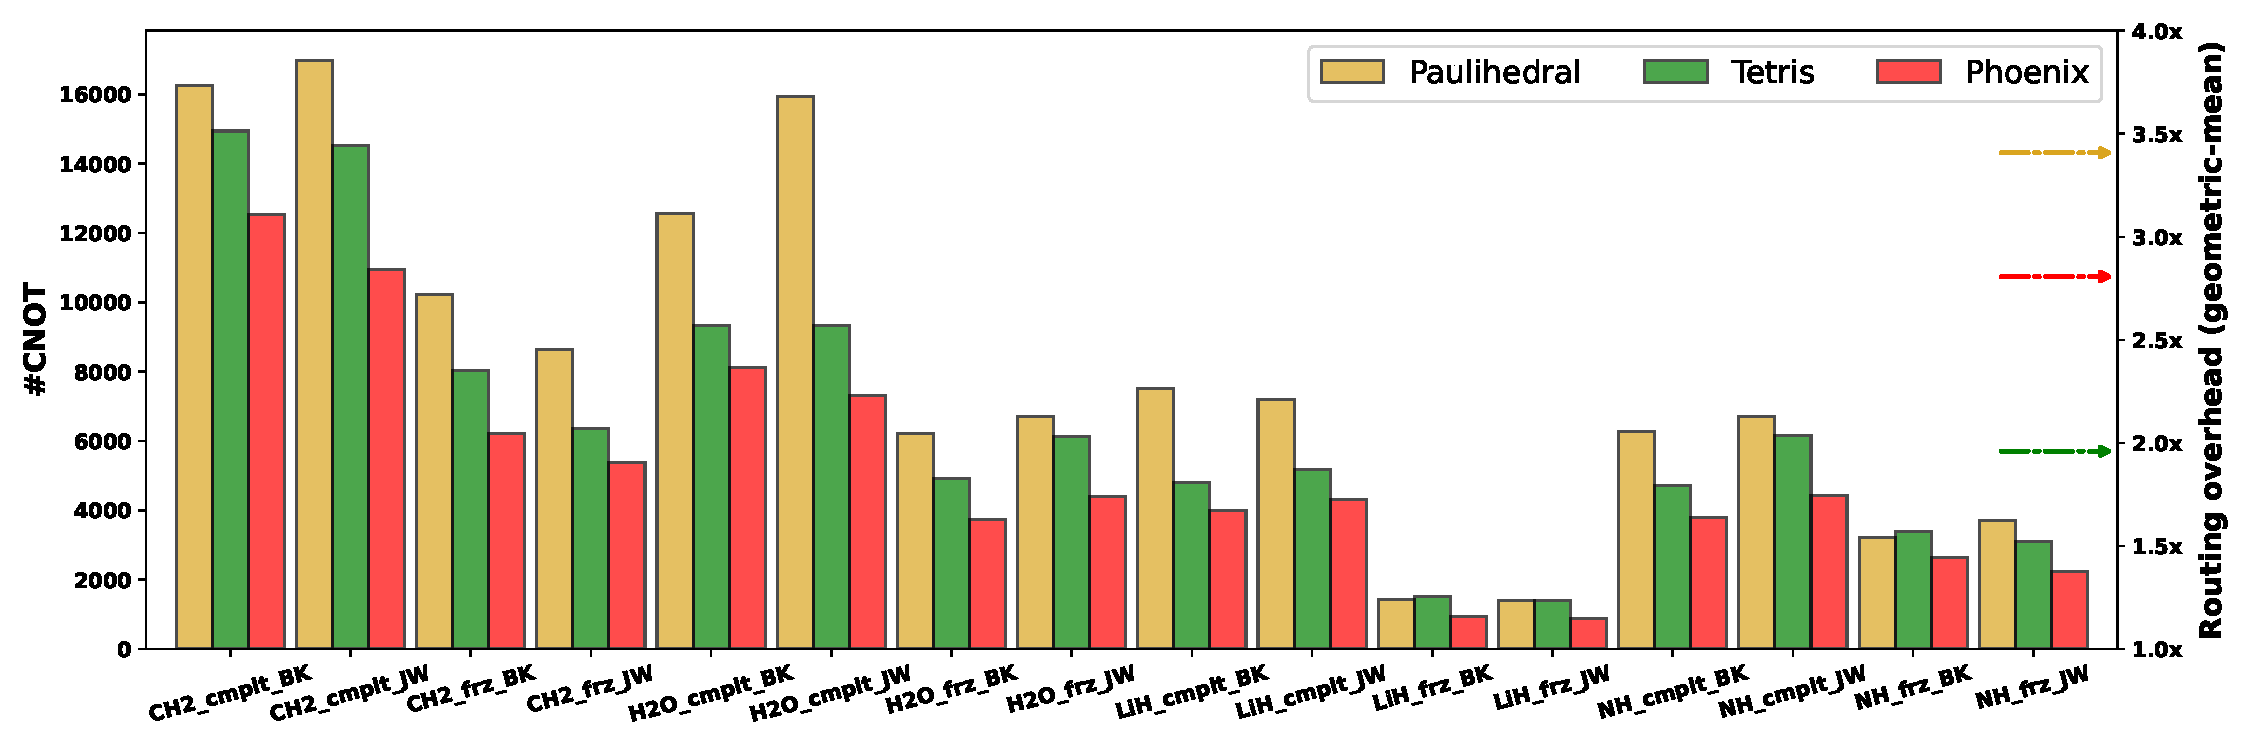
\includegraphics[width=\columnwidth]{figures/num_2q_gates_manhattan.pdf}
    \caption{Hardware-aware compilation for limited-topology NISQ device}
    \label{fig:manhattan}
\end{figure}


\begin{figure}[tbp]
    \centering
    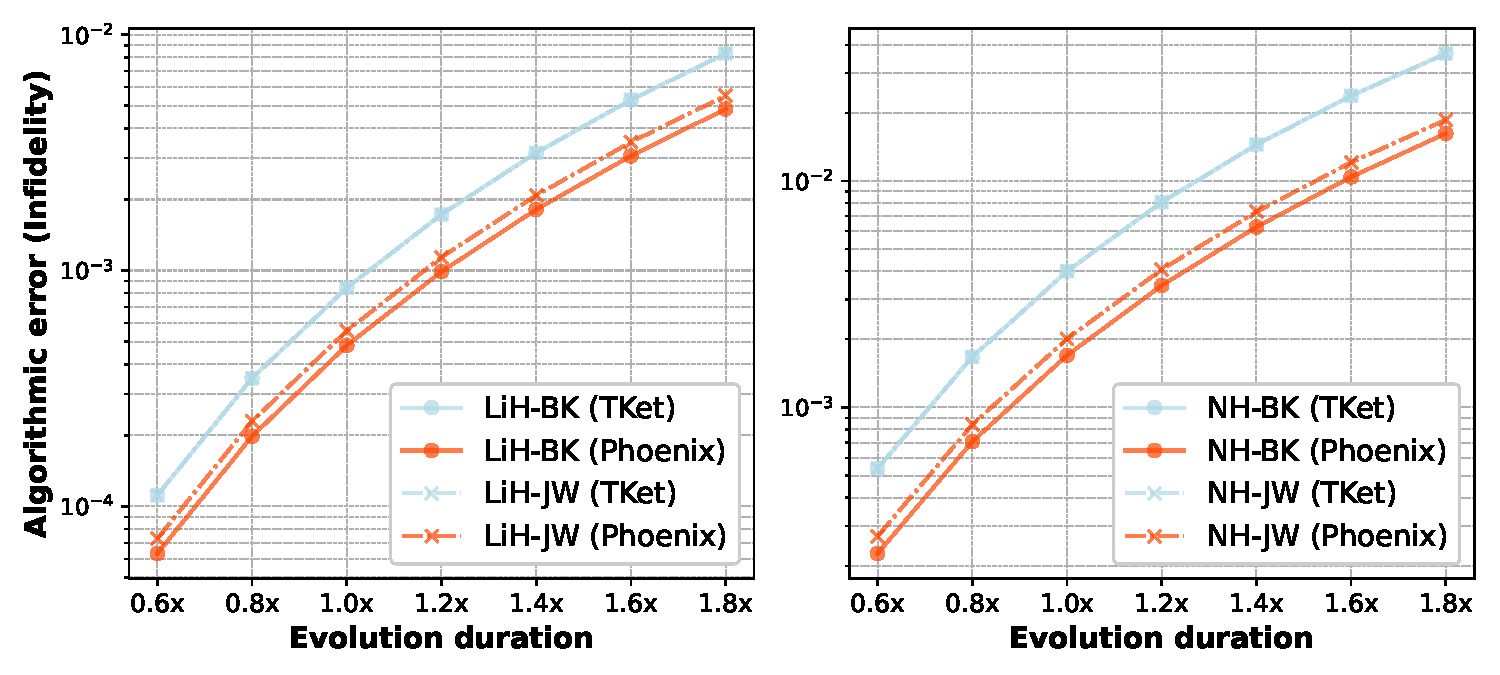
\includegraphics[width=\columnwidth]{figures/algo_err.pdf}
    \caption{Algorithmic error}
    \label{fig:algo-err}
\end{figure}




\subsection{Diverse ISA comparison}


\begin{figure}[tbp]
    \centering
    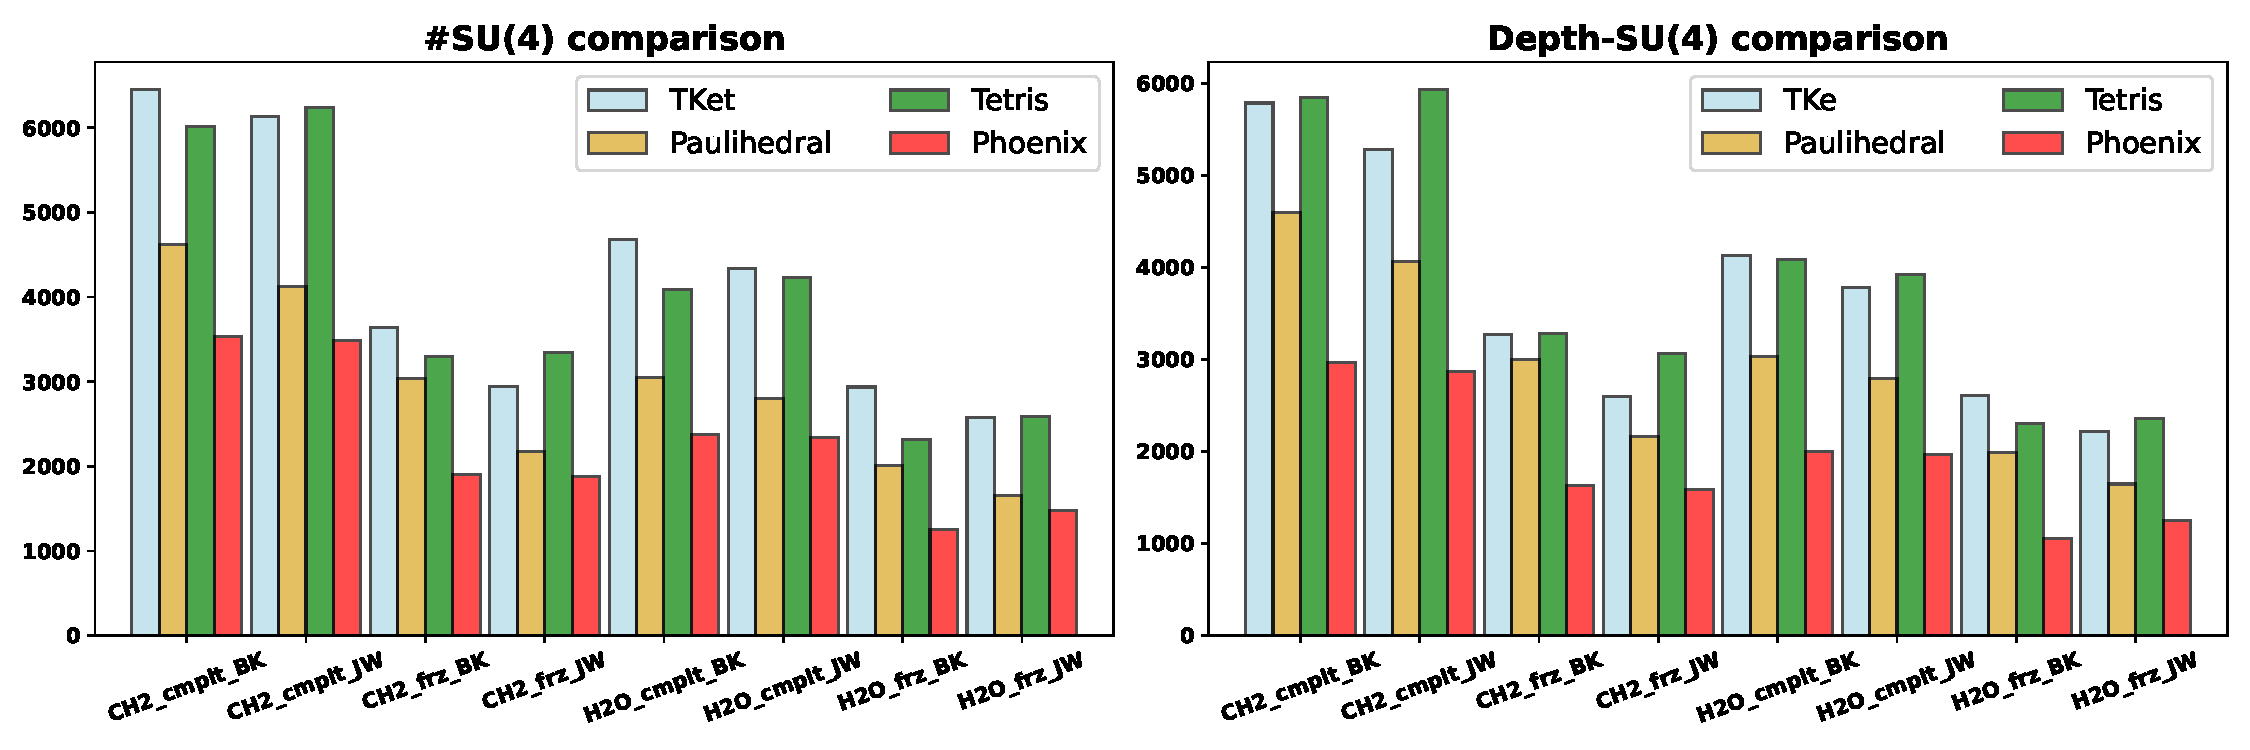
\includegraphics[width=\columnwidth]{figures/su4_comparison.pdf}
    \caption{SU(4) ISA comparison}
    \label{fig:su4-isa}
\end{figure}






\subsection{Real system evaluation}


\subsection{Scalability}







%%%%%%%%%%%%%%%%%%%%%%%%%%%%%%%%%%%%%%%%%%%%%%%%%%%%%%%%%
% Acknowledgement
%%%%%%%%%%%%%%%%%%%%%%%%%%%%%%%%%%%%%%%%%%%%%%%%%%%%%%%%%
% \section*{Acknowledgement}
% ...

%%%%%%%%%%%%%%%%%%%%%%%%%%%%%%%%%%%%%%%%%%%%%%%%%%%%%%%%%
% Reference
%%%%%%%%%%%%%%%%%%%%%%%%%%%%%%%%%%%%%%%%%%%%%%%%%%%%%%%%%

% \bibliographystyle{IEEEtran}
% \bibliography{reference}


%%%%%%%%%%%%%%%%%%%%%%%%%%%%%%%%%%%%%%%%%%%%%%%%%%%%%%%%%
% Appendix
%%%%%%%%%%%%%%%%%%%%%%%%%%%%%%%%%%%%%%%%%%%%%%%%%%%%%%%%%


% \appendix{...}




\end{document}
